\section{Introduction}


%% Background

Seizure semiology, ``the historical elicitation or observation of certain symptoms and signs'' during seizures, provides context to infer epilepsy type \cite{fisher_operational_2017}.
\Acp{FOS} start in one region of one hemisphere.
If they spread to both hemispheres, they are said to \emph{generalize}, becoming \acp{FBTCS} \cite{fisher_operational_2017}.
In \acp{FBTCS}, the patient first presents semiologies associated with a \ac{FOS}, such as head turning or mouth and hand automatisms.
This is followed by a series of phases, in which muscles stiffen (tonic phase) and limbs jerk rapidly and rhythmically (clonic phase).
\Acp{FBTCS} put patients at risk of injury and, if the seizure does not self-terminate rapidly, can result in a medical emergency.
%
% \acs{SUDEP} is the \acl{SUDEP}, without evidence of typical causes of death. \acused{SUDEP}
The risk of \ac{SUDEP} depends on epilepsy and seizure characteristics as well as living conditions.
\Acp{FBTCS} in particular increase \ac{SUDEP} risk substantially \cite{nashef_unifying_2012}.
In a small number of \ac{SUDEP} cases occurring in \acp{EMU} (32/246, i.e., 13~\%), death was preceded by a \ac{FBTCS} followed by cardiorespiratory dysfunction minutes after seizure offset \cite{ryvlin_incidence_2013}.
Identifying semiologies related to increased risk of \ac{SUDEP} to appropriately target treatment is an open research question.
One limitation determining \ac{SUDEP} risk factors is that inter-rater reliability based on qualitative visual analysis is poor for most semiological features (e.g., limb movement, head pose or eye gaze), especially between observers from different epilepsy centers \cite{tufenkjian_seizure_2012}.
Therefore, automatic and quantitative analysis of video-recorded seizures is needed to standardize assessment of seizure semiology across multicenter studies \cite{ahmedtaristizabal_automated_2017}.



%% Related works

% Other works not using deep learning
Early quantitative analysis studies of epileptic seizures evaluated patient motion by attaching infrared reflective markers to key points on the body or using cameras with color and depth streams \cite{li_z_movement_2002,cunha_movement_2003,odwyer_lateralizing_2007,cunha_neurokinect_2016}.
These methods are not robust to obscurations by bed linens or clinical staff, differences in illumination and pose, or poor video quality caused by compression artifacts or details out of focus.

% Other works using deep learning
Neural networks can overcome these challenges by automatically learning features from the training data that are more robust to variations in the data distribution.
Most related works using neural networks focus on classifying the \emph{epilepsy type} by predicting the location of the \ac{EZ}, e.g., ``temporal lobe epilepsy'' vs. ``extratemporal lobe epilepsy'', from short ($\le \SI{2}{s}$) snippets extracted from videos of one or more seizures \cite{ahmedt-aristizabal_deep_2018,ahmedt-aristizabal_hierarchical_2018,ahmedt-aristizabal_deep_2018-1,maia_epileptic_2019,karacsony_deep_2020}.
Typically, this is done as follows.
First, the bed is detected in the first frame and the entire video is cropped so the \ac{FOV} is centered on the bed.
During training, a \ac{CNN} is used to extract features from each frame in a sampled snippet.
Then, a \ac{RNN} aggregates the features into a \emph{snippet-level} representation and a fully-connected layer predicts the epilepsy type.
Finally, a \emph{subject-level} prediction is obtained by averaging all snippet-level predictions.
This approach has several disadvantages.
First, it is not robust to incorrect bed detection or changes in the \ac{FOV} due to zooming or panning.
Second, the order of semiologies is ignored, as the epilepsy type is predicted from short snippets independently of their occurrence during a seizure.
Moreover, patients with the same epilepsy type may present several seizure types.
Finally, training neural networks from small datasets, as is often the case in clinical settings, leads to limited model generalizability to new data.

The goal of this work is to compute \emph{seizure-level} representations of arbitrarily long videos when a small dataset is available for training, which is typically the case in \acp{EMU}.

% Why human action recognition models could be useful
To overcome the challenge of training with small datasets, transfer learning from \acp{STCNN} trained for \ac{HAR} can be used \cite{karacsony_deep_2020} (\cref{fig:kinetics}).
Although seizures are, strictly speaking, not actions, \ac{HAR} models are expected to encode strong representations of human motion that may be relevant for seizure characterization.
These methods are typically designed to classify human actions by aggregating predictions for snippets sampled from short clips ($\approx \SI{10}{\second}$).
Epileptic seizures, however, can last from seconds to tens of minutes \cite{jenssen_how_2006}.
A common aggregation method is to average predictions from randomly sampled snippets \cite{carreira_quo_2017,ghadiyaram_large-scale_2019,simonyan_two-stream_2014}.
Averaging predictions typically works because most video datasets considered are trimmed, i.e., the same action occurs along most of the video duration.
In our dataset, due to the nature of \acp{FBTCS}, more than half the frames are labeled as non-generalizing in 49/79 (62\%) of the \ac{FBTCS} videos.
Therefore, simply averaging snippet-level predictions would result in a large number of seizures being misclassified as \acp{FOS}.
% Why a TSN architecture helps
\Acp{TSN} \cite{wang_temporal_2019} split videos of any duration into $n$ non-overlapping segments and a consensus function aggregates features extracted from each segment.
Therefore, we propose the use of \acp{TSN} to capture semiological features across the entirety of the seizure.
We use an \ac{RNN} as a consensus function to model the sequence of feature vectors extracted from the segments.

\begin{figure}[hbt!]
  \centering
  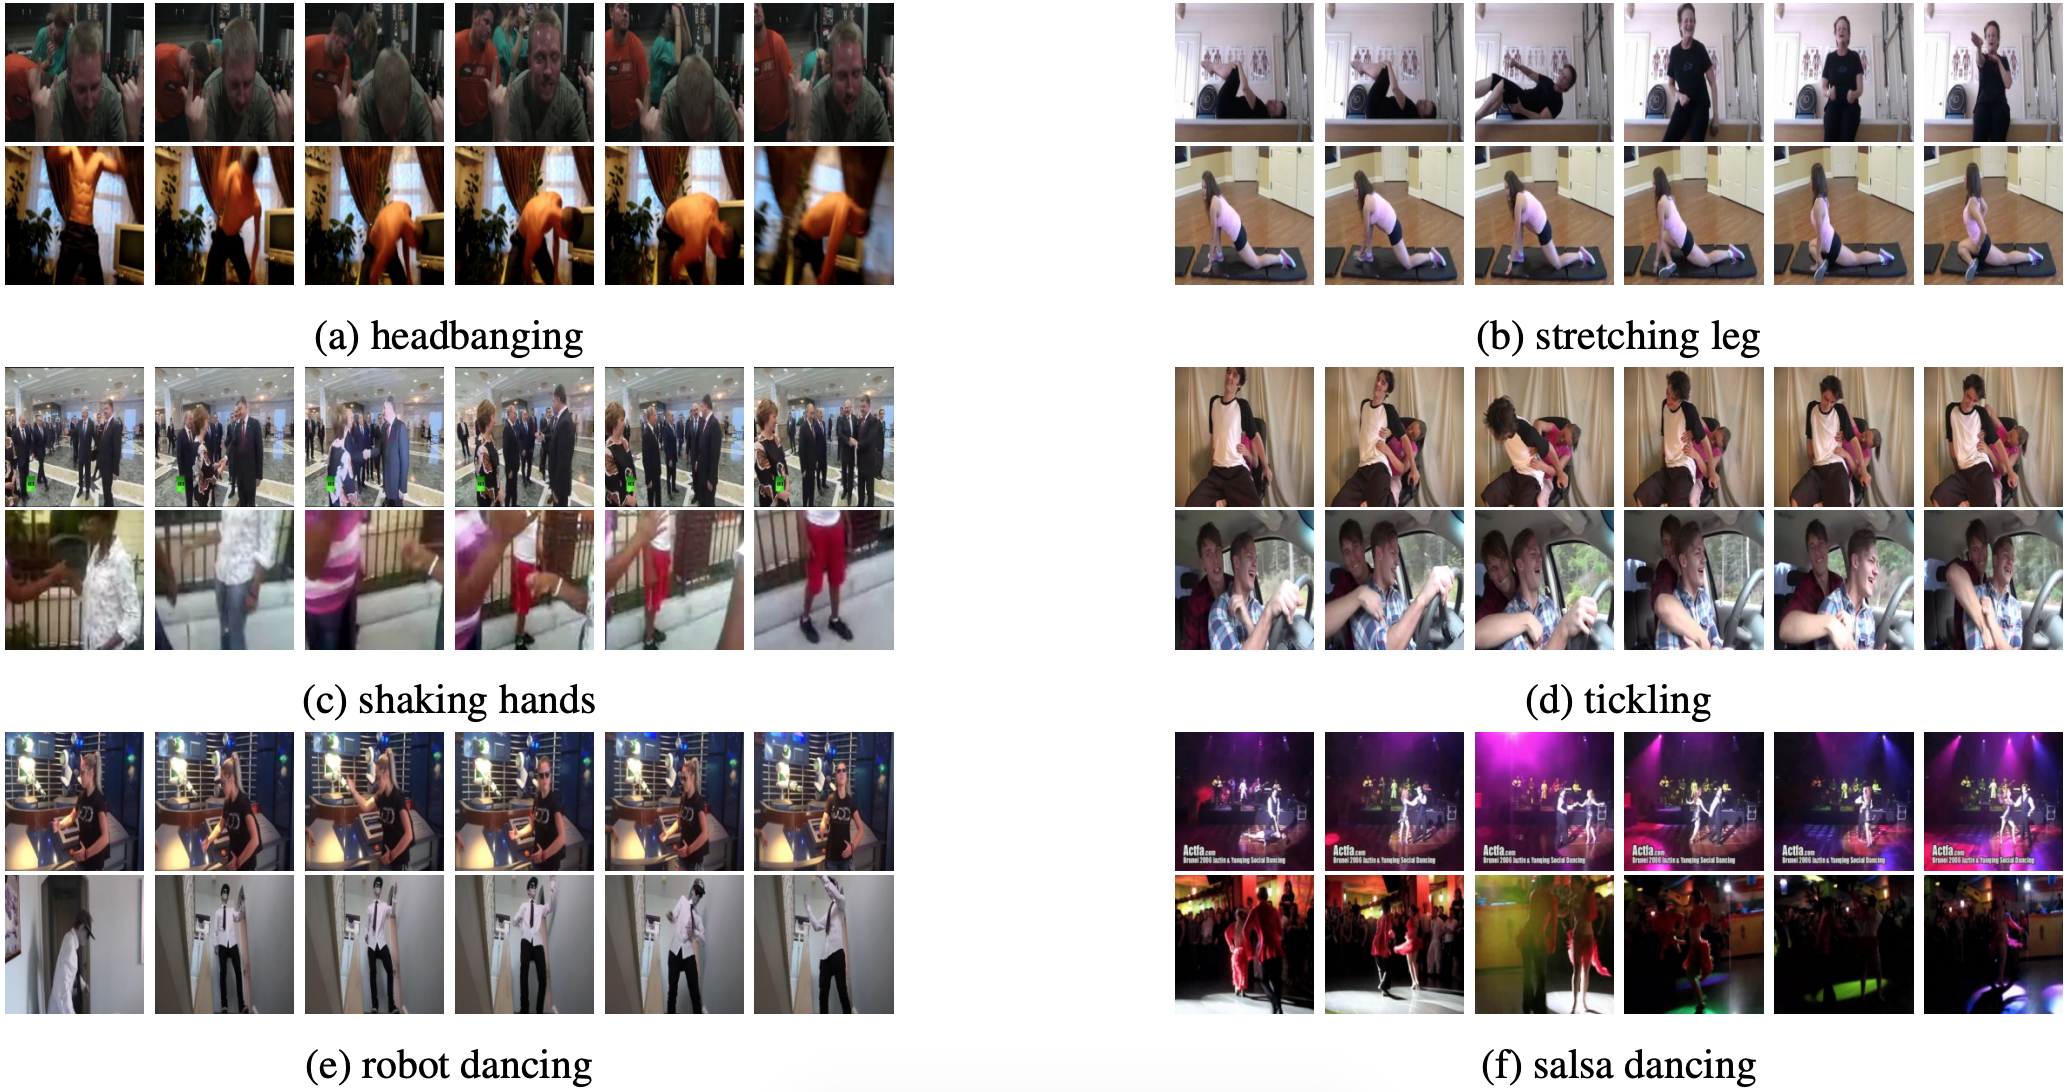
\includegraphics[width=\linewidth]{har_kinetics}
  \caption[Example classes from the Kinetics dataset]{
    Example classes from the Kinetics dataset.
    Adapted from \cite{kay_kinetics_2017}.
  }\label{fig:kinetics}
\end{figure}


% Our proposal
We present a novel neural network architecture combining \acp{TSN} and \acp{RNN}, which we denote \ac{GESTURES}, that provides full representations of arbitrarily long seizure videos.
These representations could be used for tasks such as classification of seizure types, seizure description using natural language, or triage.
To model the relevant patient motion during seizure without the need for object detection, we use a \ac{STCNN} trained on large-scale \ac{HAR} datasets (over 65 million videos from Instagram and 250,000 from YouTube) \cite{ghadiyaram_large-scale_2019} to extract features from short snippets.
Then, an \ac{RNN} is used to learn a representation for the full duration of the seizure.

% Our proof-of-concept task
We chose as a proof of concept to distinguish between \acp{FOS} and \acp{FBTCS}, because the key distinction, if the discharge spreads across hemispheres, is only observed later in the seizure.
This task demonstrates that we can train a model to take into account features across the entirety of the seizure to distinguish between seizure types.
The main challenge (even for humans), apart from the typical challenges in video-telemetry data described above, is distinguishing between \acp{FBTCS} and hyperkinetic \acp{FOS}, which are characterized by intense motor activity involving the extremities and trunk.
